\documentclass{article}
\usepackage{amsmath}  %math package for mathematical symbols and environments
\usepackage{amssymb}
\usepackage{graphicx} % Required for inserting images
\usepackage{subcaption}
% for tabs
\usepackage{booktabs} 
\usepackage{tabularx}
\usepackage{xltabular}
%
\usepackage{pgffor} % for loop
\usepackage{xstring} % for dealing with underline (_)
\usepackage{tikz} % for flowcharts 
\usetikzlibrary{shapes.geometric, arrows, arrows.meta, calc, positioning, intersections}
\usepackage{xcolor}
\usepackage{listings}
\usepackage{float}
\usepackage{adjustbox} % for fitting thing into a page
\widowpenalties 1 10000 % for not splitting acapites
\usepackage[style=apa, backend=biber]{biblatex}
\addbibresource{sources.bib}

\usepackage{datetime2}

% ---- Title / date ---
\title{Action-Grounded Symbols: Abstracting Symbols from Skills in a Mobile Robot}
\author{Klara Skorupowska}
\date{Wygenerowano: \DTMnow}

% ---- Code Listings Styles ----
% Define colors suitable for academic code listings
\definecolor{codegreen}{rgb}{0.1,0.5,0.1}
\definecolor{codepurple}{rgb}{0.5,0,0.5}
\definecolor{codeblue}{rgb}{0.1,0.2,0.7}
\definecolor{backcolour}{rgb}{0.97,0.97,0.97}

% Define PDDL language for listings
\lstdefinelanguage{PDDL}{
  sensitive=false, % PDDL is case-insensitive
  morecomment=[l]{;}, % Comments start with a semicolon
  morestring=[b]", % Strings (if any)
  % Core PDDL keywords
  morekeywords={
    define, domain, problem,
    :requirements, :types, :constants, :predicates, :functions,
    :action, :parameters, :precondition, :effect,
    :objects, :init, :goal, :metric
  },
  % Logic operators & qualifiers
  morekeywords=[2]{
    and, or, not, exists, forall, when,
    increase, decrease, total-cost
  }
}

% Global styling for listings
\lstset{
  language=PDDL,
  backgroundcolor=\color{backcolour},
  commentstyle=\color{codegreen}\itshape,
  keywordstyle=\color{codeblue}\bfseries,
  keywordstyle=[2]\color{codepurple}\bfseries,
  basicstyle=\ttfamily\footnotesize,
  breakatwhitespace=false,
  breaklines=true,
  postbreak=\mbox{\textcolor{gray}{$\hookrightarrow$}\space},
  captionpos=b,
  keepspaces=true,
  numbers=left,
  numbersep=8pt,
  numberstyle=\tiny\color{gray},
  columns=flexible
  showspaces=false,
  showstringspaces=false,
  showtabs=false,
  tabsize=2,
  frame=single,
  rulecolor=\color{lightgray}
}

% flow chart styles
% ---- Colours ----
\definecolor{orange}{HTML}{E6661A}
\definecolor{green}{HTML}{66CC66}
\definecolor{blue}{HTML}{1A80CC}
\definecolor{yellow}{HTML}{E6CC33}
\definecolor{black}{HTML}{26262E}

% ---- Flowchart Components ----
\tikzset{
    startstop/.style = {rectangle, rounded corners, minimum width=3cm, minimum height=1cm, text centered, draw=black, fill=orange!20},
    process/.style   = {rectangle, minimum width=3.5cm, minimum height=1cm, text centered, draw=black, fill=yellow!20},
    io/.style        = {trapezium, trapezium left angle=70, trapezium right angle=110, minimum width=3cm, minimum height=1cm, text centered, draw=black, fill=blue!15},
    subroutine/.style= {rectangle, draw=black, fill=yellow!20, minimum width=3.5cm, minimum height=1cm, text centered, double},
    decision/.style  = {diamond, aspect=2, minimum width=3cm, minimum height=1cm, text centered, draw=black, fill=green!20},
    arrow/.style     = {thick, ->, >=stealth}
}

\begin{document}
% ---- debug helpers ----
\newcommand{\todo}[1]{%
  \colorbox{green}{[TODO: #1]}\\%
}
\newcommand{\checkthis}[1]{
        \colorbox{yellow}{(Q: #1?)}
}

\maketitle
\newpage
\begin{center}
    \textbf{Abstract}
\end{center}
%% abstract 
\vspace{0.5cm}

\textbf{Key words:} artificial intelligence, abstract symbols, computational cognitive science

\newpage
\tableofcontents


% --- The structure ---
% Introduction: the goal, the problems, used methods, why it's important
\newpage
%% introduction
\section{Introduction}
\todo{To be addded, when body is ready}

This project is a replication of the work of \textcite{konidaris2018skills}. The project's high-level idea and philosophical problem at a basis are identical to those of Konidaris'. I introduced some minor changes to the implementation in order to facilitate replication and, at crucial aspects, get closer to biological accuracy. 

\todo{ As a result... The conclusion is...}

\subsubsection*{Paper structure} 
Chapter~\ref{chapter:theory} of this paper presents theoretical grounds, used tools, and assumptions behind this project. \\
In chapter~\ref{chapter:idea}, the algorithm is described as a high-level idea, with no implement-specific details. \\
Implementation is shown in chapter~\ref{chapter:implement}.\\
Chapter~\ref{chapter:results} shows obtained symbols, and results for completing the task, as well as learning statistics. \\
Chapter~\ref{chapter:discussion} discusses those results, and indicates future steps for this project. 

% Theory: symbol grounding problem, abstracting symbols, phylosophy and engineering
\newpage
%% theory
% the embodiment
% the symbol emergence - for action not communication
% algorithm? Konidaris 
% changes inspired by brain's biology
% -> GNG as similar came from SOM which came from bulding models of biological neural systems
% -> data from camera is preproccess using cones (RGB values) and retinal ganglion cells (edges)

\section{Theoretical Foundations} \label{chapter:theory}

% In this project, an embodied agent abstracts grounded symbols as a Growing Neural Gas (GNG) representations.
% Embodied cognition, the Symbol Grounding Problem, and the GNG algorithm have been around since the 1990s. Despite their maturity, these concepts remain relevant because Embodied Cognition was not contradicted, the Symbol Grounding Problem not solved, and even though GNG algorithm has its optimised successors, its foundational principles hold up well. I have chosen those methods to minimise the unnecessary complexity and focus on demonstrating, how abstract symbols can come from simple actions and methods. 

\subsection{Embodied Cognition} \label{chapter:theory:embodied}
% what it is
According to the movement of embodied cognition, embodiment is inseparable part of the cognition \parencite{varela2017embodied}. This stands in opposition to more classical cognitive science, representing computational theory of mind, where brain is a processor that handles abstract information \parencite{pylyshyn1984computation}. 

% characteristics that i use 
To formalise the term of embodied cognition, \textcite{Wilson2002} introduced the six views. It is six statements that define what it means for the cognition to be embodied. In the context of this project the most interesting one is the fifth, although rest of them are also fulfilled. 

\checkthis{Should I write about all six, or at least list them all?}

The fifth view: Cognition is for action. This means that the mind's function is to guide action. Every mechanism, process or representation within the mind has to come from the need of planning or executing actions. Mind's main task is to control the movement of the body in an environment and ensure its survival.

% criticism
Embodied cognition is criticized. Radical variants of embodied cognition face significant theoretical challenges. For example, by the poverty of stimulus argument, which states that there is not enough information and structure in environment to solve cognitive problems \parencite{milkowski2017situatedness}. Miłkowski settles on a hypothesis that for cognition both realms are important, embodiment and computations. Embodied experimental designs do lead to interesting discoveries, but not all cognitive processes can be explained by it. 

% how do I use it
This project focuses on what embodiment can do. Specifically, the agent learns to perceive its environment through action-oriented predicates. Each symbol emerges because some skill needs it. 

\subsection{Symbol Grounding Problem and Symbol Emergence} \label{chapter:theory:SGP}
% what it is
Symbol Grounding Problem (SGP) was introduced by \textcite{harnad1990symbol}. His starting point is computational theory of mind that looks at a brain as open-loop computing machine that operates within symbol systems. He drew attention to the meanings of those symbols, arguing that any interpretation for them, must be extrinsic to the system. He compares understanding such symbols to learning Chinese solely from the Chinese dictionary. Every attempt to find a meaning leads only to more symbols, that still lack the meaning. The Grounding Problem asks the question if there is a mechanism that allows finding the meanings of symbols without escaping the system, therefore making them intrinsic to it. This is one side of the problem, in a context of robotics and cognitive modelling, the essential challenge is not only symbol grounding but also symbol emergence: not only how to find the meaning of existing symbols, but how meaningful symbols arise, evolve, and become organized through social and embodied interaction \parencite{taniguchi2016symbol}.

% characteristics that i use
Harnad himself proposed a solution to SGP \parencite{harnad1990symbol}. The mind grounds symbols in environment by creating iconic or categorical representations. It is a mechanism of associating the sensations with objects causing them. An object is then described in terms of sensory projection: as a representative point in perceptual space (an icon) or multiple points' invariants (a category). Even though, Harnad do not point out what triggers this mechanism, Peirce’s pragmatism effectively addresses this issue. It ties objects and their characteristics with actions they are associated with \parencite{kato2026pragmatism}. 

% criticism
This and other solutions, from different angles, were proposed, yet the problem remain opened. \textcite{taddeo2005solving} conducted a review of 15 years of solving the SGP. They concluded that explanations rely on pre-installed or other way given semantic resources. 

% how do I use it
This project likewise depends on external structures and symbol manipulation. The skills and actions are pre-coded, but symbols emerge. Those symbols, essential for operating within an environment, are obtained by repetitive discovery of possible sensory projections and binding them to the actions, they are not pre-installed but learned through interaction with an environment. The symbols are then used for planning and executing a task using planning algorithms.

\subsection{Sensory Input: Visual Processing} \label{chapter:theory:visuals}
Biological sensory input is processed through neural paths before it reaches the brain. Even there, this early processed input can be further manipulated. \parencite{crick2003framework}. The robot under consideration has two types of sensors: LIDARs and RGB camera. Since humans do not possess anything remotely like the LIDARs, I focus on the vision.

% what it is
The subject of recognising colours is described by \textcite{livingstone1988segregation}. They described how the eyes and the brain analyse visual input. Colour is perceived by the cells in the retina called cones. There are three types of cones: red-, green- and blue-sensitive. This is enough to distinguish between colours. 

Another type of processing that happens at retinal level is detecting the differences in light saturation. They allow us to see the edges of objects in our visual field. Those cells are called retinal ganglion cells, and they form receptive fields. A receptive field has two areas: the on-centre and the off-centre. If the on-centre cells perceive more photons than the off-centre ones, the on-centre is activated. If the off-centre perceives more, the off-centre is activated. If both perceive the same amount, there is no activation \parencite{kuffler1953discharge}.

% criticism
Kuffler assumed some things that were proven wrong. First example is the linearity of the ganglion cell receptive fields. \textcite{enroth1966contrast} proved that this is an oversimplification. Complete linearity means that the linear change in lighting is translated to the linear reaction of the cells in full input range. Yet some receptive fields are more sensitive to darkness, some to brightness. 

Another example of known flaw in Kuffler’s model is the laboratory setting of creating it. Keffler used tiny spots of light on anesthetised cat’s retina. Yet in natural condition, the lighting changes, the eye moves. Later it was proven that the receptive fields adapt dynamically to those changing conditions \parencite{smirnakis1997adaptation}.

% characteristics that i use 
Even though Keffler's model is a huge oversimplification, it is still a basis for the next models. I decided to use a simple model in this project, since it is a proof of concept.

% how do I use it
For this project, the visual information from RGB camera matrix is translated to activation of red, blue, and green cones, and activation of on-centre and off-centre fields. Such pre-processed visual information is passed further to the symbol emergence algorithm. 

\subsection{Symbol Representation: Growing Neural Gas} \label{chapter:theory:GNG}
% what it is
Symbolic representations describe raw sensory input in a more abstract way enabling reasoning, planning, and acting. In the philosophy of mind, the ontological status of representations is a subject of debate. \textcite{fodor1975language} proposed that the mind is a symbolic system, and that mental representations are symbolic. \textcite{smolensky1988proper} argued that those representations are not symbolic, but rather subsymbolic. In this connectionists view, representations are not discrete symbols, but rather continuous patterns of activation in neural networks. Radical anti-representationalists and enactive paradigms argue that the thoughts are neither symbolic nor subsymbolic, but rather non-representational. They are patterns of sensorimotor activity \parencite{brooks1991intelligence}. 

% characteristics that i use
This work assumes that the representations are subsymbolic. The representations can be presented as a topological map of the perceptual space and manipulated in a symbolic manner.

% the math / computer science
A well-established algorithm for creating topological maps is the Self-Organizing Map (SOM) algorithm.\parencite{ritter1989som, kohonen1982self}. It assumes fixed structure of the map, such as a grid. Then it is trained to represent the input space by adjusting positions of the existing nodes. The Growing Neural Gas (GNG) algorithm \parencite{fritzke1994gng} extends the SOM framework. It does not assume a predefined structure. It starts with two nodes, grows by adding new ones in areas of high error, and removes ones in unvisited areas. This allows the GNG to adapt to the input space and represent it more accurately.

% how do I use it
In this project, the GNG algorithm encodes sensory observations corresponding to successful executions of skills. Then, symbols relevant for the task are abstracted through the mathematical operations on these topological maps.

% The idea: the high level idea, where ideas are from
\newpage
\section{High-Level Idea} \label{chapter:idea}

\subsection{\checkthis{The Story}}
Imagine an embodied agent - a robot. We want it to complete a task for us. It has a library of ready-to-use skills. To complete the task, the robot needs to execute those skills in correct order. But, for slightly different task, or in different circumstances, some skills may be unnecessary, or the order needs to be changed. We want our robot to smoothly adapt to the changes in an environment and given objectives, and only focus on what is important for a specific skill. 

Take a closer look at the skills. A skill is a list of low-level actions, that can be executed by this robot. Their execution ends either successfully, or fail at some action. Obviously, the robot should execute a skill only when it can assume that the execution is going to be successful. For that each one comes with a precondition. A precondition is a symbol, or conjunction of them, that says "You can do this skill now". These symbols are predicates resolvable by examining the perceptual state of the robot. Robot can take a look around and decide if a skill is save to execute. Then, after skill execution, the robot changes its perceptual state, either by changing something in the environment or changing its location. This new state is another predicate: an effect. Since the robot is supposed to execute skills successfully, only effects of those are of any interest to it. Then robot uses those predicates to establish which skills need to be done, and in which order to complete assigned task. The aim of this project is to let the robot learn those predicates on its own.

\subsection{Starting Point}
This is a replication of the work of \textcite{konidaris2018skills}. They proposed a framework for abstracting grounded symbols from predefined skills. Their framework collected data from repetitions of skills. It saves initial and final states in a form of 3D representation as cloud of points. Then, it uses clustering methods, such as DB-SCAN to find what the skill changes in the environment. In the learning setting, the robot had two arms, a mobile platform, and a binocular vision. The task setting was a room with a bottle in a closed fridge and a closed cupboard. The task for the robot was to move a bottle from the fridge to the cupboard. In a learning phase, the skills, such as opening the fridge, were repeatedly executed, starting from a known initial state. The learning data consisted only of successfully completed trials. Then they used the clustering algorithm to find clusters of repetitive patterns through all the repetitions. This way they obtained symbols that could be interpreted, for example, as "Fridge is open", or "robot is holding the bottle". 

Starting from this framework, this project aims to abstract symbols continuously, without seperating learning and exploiting phases. Additionally, some changes are made in the data collection and abstraction methods to make them more biologically accurate.

\subsection{Algorithm Description}

In contrast to the original work, this framework runs uninterrupted, continuously trying to finish the given task. As a part of the mechanism, obtaining symbols will enable it to do so. Figures \ref{fig:flow_mainloop} to \ref{fig:flow_generate_plan} show the logic of the most important processes within the framework. The learning and exploiting phases are intertwined into the main loop of the program.

The learning process is partially supervised. The execution of skills is evaluated externally by the Supervisor. The supervisor does not interfere with the symbol abstracting mechanism but rather is a guide whether the outcome is desirable or not.

The exploiting process is based on the PDDL language. The agent generates a plan based on the current state of the environment and the learned symbols. Then, it executes the plan step by step, while continuously checking if the execution is successful. If not, it explore by executing random skill, and tries to generate a new plan.

\begin{figure}[htbp]
    \centering
    \adjustbox{max width=\textwidth, max totalheight=0.85\textheight, keepaspectratio}
    {
        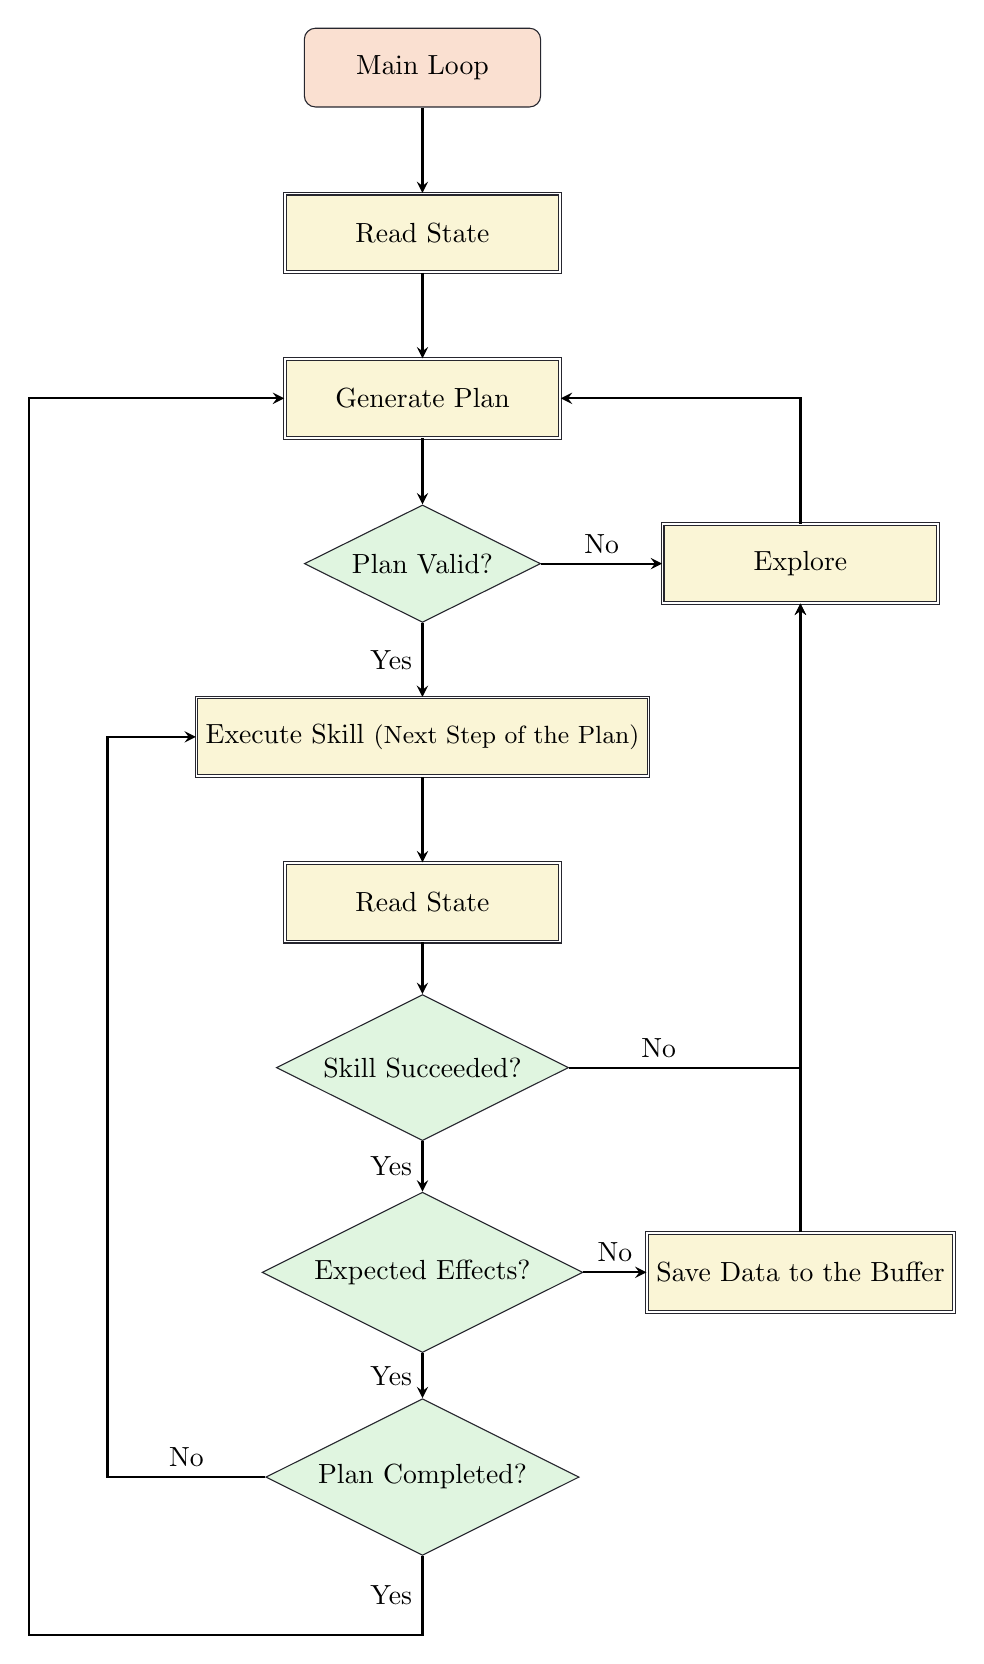
\begin{tikzpicture}[node distance=1.6cm]

\node (start) [startstop] {Main Loop};

\node (read_state1) [subroutine, below of=start, yshift=-0.5cm] {Read State};

\node (gen_plan) [subroutine, below of=read_state1, yshift=-0.5cm] {Generate Plan};

\node (plan_valid) [decision, below of=gen_plan, yshift=-0.5cm] {Plan Valid?};

\node (explore) [subroutine, right of=plan_valid, xshift=3.2cm] {Explore};

\node (exec_step) [subroutine, below of=plan_valid, yshift=-0.6cm] {Execute Skill \small{(Next Step of the Plan)}};

\node (read_state2) [subroutine, below of=exec_step, yshift=-0.5cm] {Read State};

\node (check_success) [decision, below of=read_state2, yshift=-0.5cm] {Skill Succeeded?};

\node (effects_there) [decision, below of=check_success, yshift=-1cm] {Expected Effects?};

\node (save) [subroutine, right of=effects_there, xshift=3.2cm] {Save Data to the Buffer};

\node (more_steps) [decision, below of=effects_there, yshift=-1cm] {Plan Completed?};

% Arrows - Loop initiation
\draw [arrow] (start) -- (read_state1);
\draw [arrow] (read_state1) -- (gen_plan);

% Arrows - Plan validation
\draw [arrow] (gen_plan) -- (plan_valid);
\draw [arrow] (plan_valid) -- node[anchor=south] {No} (explore);
\draw [arrow] (explore) |- (gen_plan.east);
\draw [arrow] (plan_valid) -- node[anchor=east] {Yes} (exec_step);

% Arrows - succeed
\draw [arrow] (exec_step) -- (read_state2);
\draw [arrow] (read_state2) -- (check_success);
\draw [arrow] (check_success) -- ++(3cm, 0) node[anchor=south] {No} -| (explore);
\draw [arrow] (check_success) -- node[anchor=east] {Yes} (effects_there);

% Arrows - expected effects
\draw [arrow] (effects_there) -- node[anchor=south] {No} (save);
\draw [arrow] (save) -- (explore.south);
\draw [arrow] (effects_there) -- node[anchor=east] {Yes} 
(more_steps);

% Arrows - plan completed
\draw [arrow] (more_steps) -- node[anchor=south] {No} ++(-4cm, 0)
              |- (exec_step.west);
\draw [arrow] (more_steps.south) -- node[anchor=east] {Yes} ++(0, -1cm) -- ++(-5cm, 0)
              |- (gen_plan.west);

\end{tikzpicture}
    }
    \caption{A flowchart of the main loop of the program. The agent continuously tries to generate a plan and execute it. If the execution fails, it explores by executing a random skill.} 
    \label{fig:flow_mainloop}
\end{figure}

\begin{figure}[htbp]
    \centering
    \adjustbox{max width=\textwidth, max totalheight=0.85\textheight, keepaspectratio}
    {
        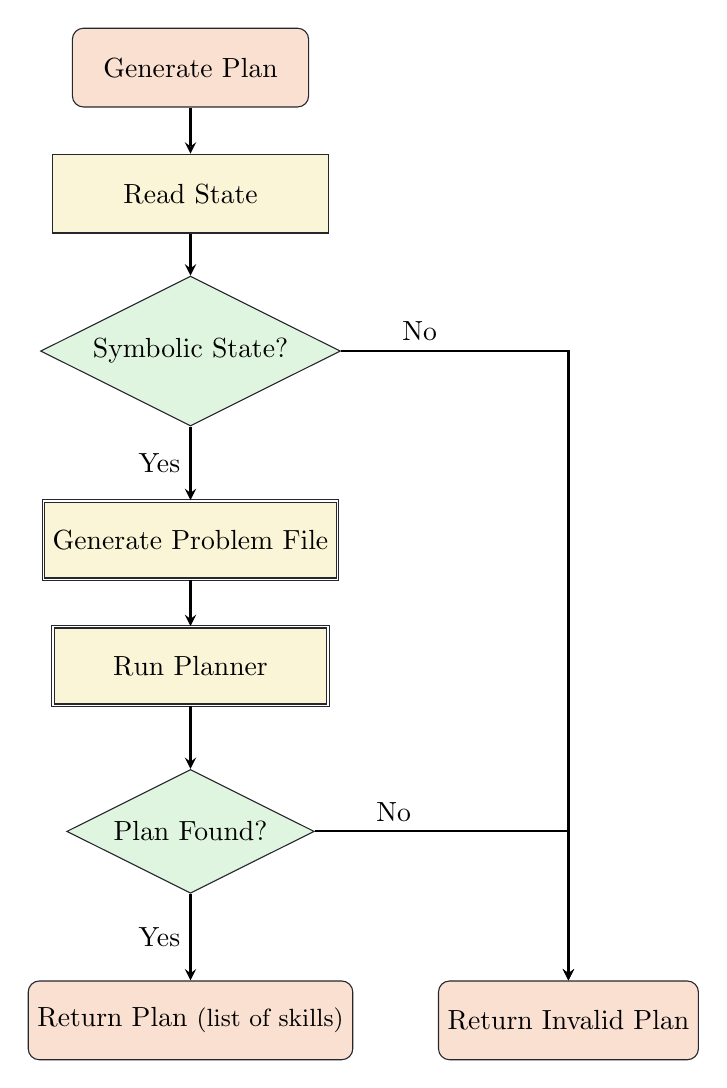
\begin{tikzpicture}[node distance=1.6cm]

% nodes
\node (start) [startstop] {Generate Plan};

\node (read_state) [process, below of=start] {Read State};

\node (active_predicates) [decision, below of=read_state, yshift=-0.4cm] {Symbolic State?};

\node (generate_problem) [subroutine, below of=active_predicates, yshift=-0.8cm] {Generate Problem File};

\node (plan) [subroutine, below of=generate_problem] {Run Planner};

\node (done) [decision, below of=plan, yshift=-0.5cm] {Plan Found?};

\node (read_plan) [startstop, below of=done, yshift=-0.8cm] {Return Plan \small{(list of skills)}};

\node (fail) [startstop, right of=read_plan, xshift=3.2cm] {Return Invalid Plan};

% arrows
\draw [arrow] (start) -- (read_state);
\draw [arrow] (read_state) -- (active_predicates);

\draw [arrow] (active_predicates) -- node[anchor=east] {Yes} (generate_problem);
\draw [arrow] (active_predicates.east) -- node[anchor=south] {No} ++(2cm,0) -| (fail.north);

\draw [arrow] (generate_problem) -- (plan);
\draw [arrow] (plan) -- (done);
\draw [arrow] (done) -- node[anchor=east] {Yes} (read_plan);
\draw [arrow] (done.east) -- node[anchor=south] {No} ++(2cm,0) -| (fail.north);

\end{tikzpicture}
    }
    \caption{A flowchart of the plan generation process. The agent attempts to generate a valid plan based on the current state and learned symbols.} 
    \label{fig:flow_generate_plan}
\end{figure}

\begin{figure}[htbp]
    \centering
    \adjustbox{max width=\textwidth, max totalheight=0.85\textheight, keepaspectratio}
    {
        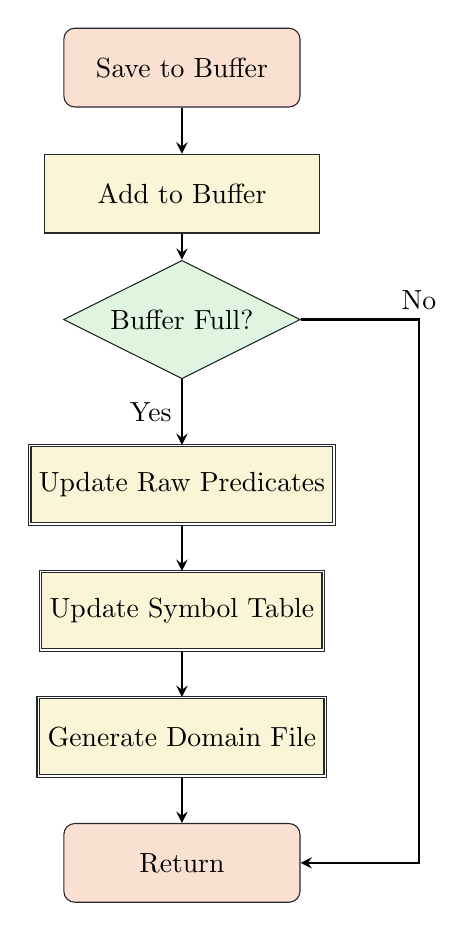
\begin{tikzpicture}[node distance=1.6cm]
% nodes
\node (start) [startstop] {Save to Buffer};

\node (add_to_buffer) [process, below of=start] {Add to Buffer};

\node (full) [decision, below of=add_to_buffer] {Buffer Full?};

\node (update_predicates) [subroutine, below of=full, yshift=-0.5cm] {Update Raw Predicates};

\node (update_symbols) [subroutine, below of=update_predicates] {Update Symbol Table};

\node (generate_domain) [subroutine, below of=update_symbols] {Generate Domain File};

\node (end) [startstop, below of=generate_domain] {Return};

%arrows
\draw [arrow] (start) -- (add_to_buffer);
\draw [arrow] (add_to_buffer) -- (full);
\draw [arrow] (full.east) -- ++(1.5,0) node[anchor=south] {No} -- ++(0,-3.2) |- (end.east);
\draw [arrow] (full.south) -- node[anchor=east] {Yes} (update_predicates.north);
\draw [arrow] (update_predicates) -- (update_symbols);
\draw [arrow] (update_symbols) -- (generate_domain);
\draw [arrow] (generate_domain) -- (end);

\end{tikzpicture}
    }
    \caption{A flowchart of the data saving process. The agent saves the initial and final states of a skill execution into a buffer for later symbol abstraction. Once the buffer is full, the agent triggers the symbol abstraction process.} 
    \label{fig:flow_save2buffer}
\end{figure}

\begin{figure}[htbp]
    \centering
    \adjustbox{max width=\textwidth, max totalheight=0.85\textheight, keepaspectratio}
    {
        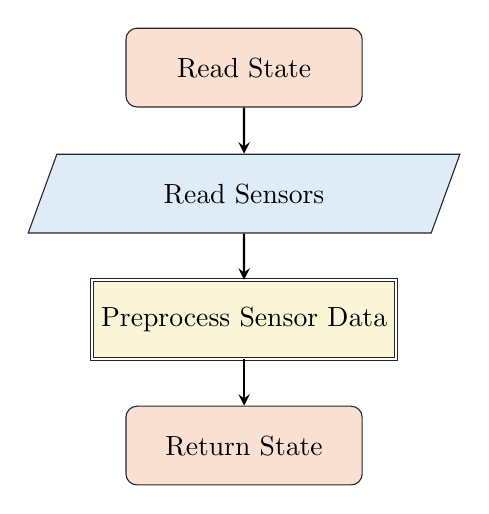
\begin{tikzpicture}[node distance=1.6cm]

\node (start) [startstop] {Read State};

\node (read_sensors) [io, below of=start] {Read Sensors};

\node (preprocess) [subroutine, below of=read_sensors] {Preprocess Sensor Data};

\node (stop) [startstop, below of=preprocess] {Return State};

\draw [arrow] (start) -- (read_sensors);
\draw [arrow] (read_sensors) -- (preprocess);
\draw [arrow] (preprocess) -- (stop);

\end{tikzpicture}

    }
    \caption{A flowchart of the state reading process. The agent reads the current state of the environment. A state is dually represented as a vector in perceptual space and as a set of active abstract symbols.} 
    \label{fig:flow_read_state}
\end{figure}

\subsubsection*{First Loops}
During first few loops, the robot has no knowledge about the environment at all. There are no raw predicates nor any abstract symbols. The program starts with an attempt to generate plan (fig. \ref{fig:flow_mainloop}). It tries to solve a task, but since the state described by symbols is empty, it fails (fig. \ref{fig:flow_generate_plan}). No valid plan to execute means exploring. Exploring is done by executing a random skill from a given skillset. If the execution is successful, the data is saved (fig. \ref{fig:flow_save2buffer}). This way the robot collects information about how the skills interfere with the environment, and what can be done using them. After a few explorations and collecting enough data, it is possible to form a predicate. This predicate is an object in perceptual space that represent the “before” or “after” of the skill. Abstracting symbols partition these objects into pieces relevant for different skills. Once the influence of the skills on the environment is established, the robot can use the abstract symbols in planning and manage the task.

\subsubsection*{Adding New Skills}
Let us assume that we have fully working abstract model of skill-environment interactions for a skillset. Expanding a skillset do not interfere with learned symbols as they are all independent. Robot need to go through exploring to abstract symbol for the new skill and update partitioning of symbols for other skills. It is also possible to manually insert existing symbols into preconditions and effects of a new skill. This way, the skillset can be expanded without additional learning.

\subsubsection*{New Elements in Environment}
Since there is no exploring and exploiting phases. In a new environment, the robot smoothly goes back to more frequent exploring. After enough experiences, the new symbols emerge. They describe the interactions between the skills and the current environment. The previously gathered knowledge is not erased, as the new experiences occure in unexplored corners of perceptual space. These new experiences expand the shape of representations, not replace them. The robot can operate in both environments. The knowledge is lost only for no longer visited areas of perceptual space. The robot forgets the knowledge about the environment that is no longer relevant for the task. 

\subsection{Abstracting Symbols}
Abstracting symbols is a mathematical operation on sets of points in perceptual space. Figure \ref{fig:abstracting_symbols} shows the process of abstracting symbols. The symbol is a region in perceptual space that was changed by the skill. For example, if the skill is to push a door open, the initial states are all the states where the robot is in front of the door, and the effect states are all the states where the robot is in the next room. Execution of the skill changes, for example, the distance between the robot and the door, and colors in the vision. Each point may differ slightly, as the execution is possible from different positions. The algorithm finds the common features of those points and abstracts them into a precondition symbol. The effect symbol is a representation of the skill's effect on the environment, obtained as the intersection of the effect states. Additionally, algorithm finds the overlapping features of precondition and effect symbols, and removes them from both. This way, the symbols are mutually disjoint, and only the features that are changed by the skill remain. Lastly, the symbols are partitioned into disjoint sets, so they can be used in symbolic planning.

\begin{figure}[htbp]
    \centering
    \adjustbox{max width=\textwidth, max totalheight=0.85\textheight, keepaspectratio}
    {
        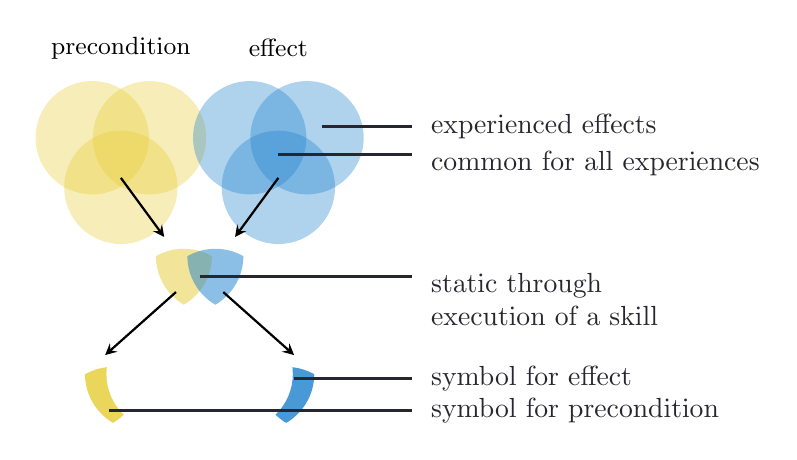
\begin{tikzpicture}[
    pointer/.style={line width=1pt, black},
    % Reusable 3-circle Venn geometry (takes radius and offset as arguments or macros)
    venn3/.pic={
        \fill (150:\vennOffset) circle (\vennRadius);
        \fill (30:\vennOffset)  circle (\vennRadius);
        \fill (270:\vennOffset) circle (\vennRadius);
    }
]
    % --- 0. LAYOUT & GEOMETRY PARAMETERS ---
    % Circle geometry
    \pgfmathsetmacro{\vennRadius}{0.72}
    \pgfmathsetmacro{\vennOffset}{0.42}
    
    % Vertical row positions (Y)
    \pgfmathsetmacro{\rowOneY}{0.0}
    \pgfmathsetmacro{\rowTwoY}{-1.5}
    \pgfmathsetmacro{\rowThreeY}{-3.0}
    
    % Horizontal positions & offsets (X)
    \pgfmathsetmacro{\leftColX}{0.0}
    \pgfmathsetmacro{\rightColX}{2.0}
    \pgfmathsetmacro{\centerX}{(\leftColX + \rightColX)/2}
    
    \pgfmathsetmacro{\midOverlapOffset}{0.2}  % Distance from centerX for row 2
    \pgfmathsetmacro{\botSpreadOffset}{1.1}   % Distance from centerX for row 3
    \pgfmathsetmacro{\diffShift}{1.0}         % Subtraction cutout shift in row 3
    \pgfmathsetmacro{\calloutX}{3.7}          % X-alignment for right-side text labels

    % Define center coordinates for every element
    \coordinate (top_left)  at (\leftColX, \rowOneY);
    \coordinate (top_right) at (\rightColX, \rowOneY);
    
    \coordinate (mid_left)  at (\centerX - \midOverlapOffset, \rowTwoY);
    \coordinate (mid_right) at (\centerX + \midOverlapOffset, \rowTwoY);
    \coordinate (mid_center) at (\centerX, \rowTwoY);
    
    \coordinate (bot_left)  at (\centerX - \botSpreadOffset, \rowThreeY);
    \coordinate (bot_right) at (\centerX + \botSpreadOffset, \rowThreeY);


    % --- 1. TOP ROW: PRECONDITION & EFFECT VENN DIAGRAMS ---
    \node[font=\small] at ([yshift=1.35cm]top_left) {precondition};
    \pic[fill=yellow, fill opacity=0.35] (pre_venn) at (top_left) {venn3};

    \node[font=\small] at ([yshift=1.35cm]top_right) {effect};
    \pic[fill=blue, fill opacity=0.35] (eff_venn) at (top_right) {venn3};


    % --- 2. MIDDLE ROW: OVERLAPPING INTERSECTIONS ---
    \begin{scope}[shift={(mid_left)}]
        \clip (150:\vennOffset) circle (\vennRadius);
        \clip (30:\vennOffset)  circle (\vennRadius);
        \fill[yellow, fill opacity=0.5] (270:\vennOffset) circle (\vennRadius);
    \end{scope}

    \begin{scope}[shift={(mid_right)}]
        \clip (150:\vennOffset) circle (\vennRadius);
        \clip (30:\vennOffset)  circle (\vennRadius);
        \fill[blue, fill opacity=0.5] (270:\vennOffset) circle (\vennRadius);
    \end{scope}


    % --- 3. BOTTOM ROW: SET DIFFERENCES (SYMBOLS) ---
    % Left: Yellow intersection minus Blue intersection
    \begin{scope}[shift={(bot_left)}]
        \clip (150:\vennOffset) circle (\vennRadius);
        \clip (30:\vennOffset)  circle (\vennRadius);
        \clip (270:\vennOffset) circle (\vennRadius);
        \begin{scope}[shift={(\diffShift, 0)}, even odd rule]
            \clip (-2,-2) rectangle (2,2) (150:\vennOffset) circle (\vennRadius);
            \fill[yellow, fill opacity=0.8] (-2,-2) rectangle (2,2);
        \end{scope}
    \end{scope}

    % Right: Blue intersection minus Yellow intersection
    \begin{scope}[shift={(bot_right)}]
        \clip (150:\vennOffset) circle (\vennRadius);
        \clip (30:\vennOffset)  circle (\vennRadius);
        \clip (270:\vennOffset) circle (\vennRadius);
        \begin{scope}[shift={(-\diffShift, 0)}, even odd rule]
            \clip (-2,-2) rectangle (2,2) (30:\vennOffset) circle (\vennRadius);
            \fill[blue, fill opacity=0.8] (-2,-2) rectangle (2,2);
        \end{scope}
    \end{scope}


    % --- 4. FLOW ARROWS (Relative to centers) ---
    \draw[arrow] ([yshift=-0.30cm]top_left)  -- ([xshift=-0.25cm, yshift=0.45cm]mid_left);
    \draw[arrow] ([yshift=-0.30cm]top_right) -- ([xshift=0.25cm,  yshift=0.45cm]mid_right);

    \draw[arrow] ([xshift=-0.10cm, yshift=-0.25cm]mid_left)  -- ([xshift=-0.10cm, yshift=0.45cm]bot_left);
    \draw[arrow] ([xshift=0.10cm,  yshift=-0.25cm]mid_right) -- ([xshift=0.10cm,  yshift=0.45cm]bot_right);


    % --- 5. CALLOUT POINTERS & LABELS (Relative to centers) ---
    \coordinate (p1) at ([xshift=0.55cm, yshift=0.35cm]top_right);
    \draw[pointer] (p1) -- (p1 -| \calloutX, 0) 
        node[right, align=left, xshift=3pt] {experienced effects};
    
    \coordinate (p2) at (top_right);
    \draw[pointer] (p2) -- (p2 -| \calloutX, 0) 
        node[right, align=left, anchor=north west, yshift=5pt, xshift=3pt] {common for all experiences};
    
    \coordinate (p3) at ([yshift=-0.05cm]mid_center);
    \draw[pointer] (p3) -- (p3 -| \calloutX, 0) 
        node[right, align=left, anchor=north west, yshift=5pt, xshift=3pt] {static through\\ execution of a skill};
    
    \coordinate (p4) at ([xshift=0.10cm, yshift=0.15cm]bot_right);
    \draw[pointer] (p4) -- (p4 -| \calloutX, 0) 
        node[right, align=left, xshift=3pt] {symbol for effect};
    
    \coordinate (p5) at ([xshift=-0.05cm, yshift=-0.25cm]bot_left);
    \draw[pointer] (p5) -- (p5 -| \calloutX, 0) 
        node[right, align=left, xshift=3pt] {symbol for precondition};
    
\end{tikzpicture}
    }
    \caption{An ideogram of the symbol abstraction process. The abstraction relies on finding common features of experience points and abstracts them into precondition and effect symbols. Symbols show the skill-environment interaction.} 
    \label{fig:abstracting_symbols}
\end{figure}

Formally, the abstraction algorithm is described as follows.

The robot collects \textit{experiences}. An experience is a triple consisting of a \textit{precondition}, a \textit{skill}, and an \textit{effect}. The precondition and effect are vectors in a continuous perceptual space $\mathcal{S}$, while the skill is a discrete label representing the action executed between them. An experience is recorded in two situations: upon successful execution of a skill during exploration, or during plan execution when the resulting effect differs from the expected one. Experience is defined as follows:

\begin{equation} \label{eq:experience}
    \text{Exp}_k^{A_i} = (s_{\text{init}, k}, A_i, s_{\text{eff}, k})
\end{equation}
\noindent\small
\begin{tabularx}{\textwidth}{@{}l@{\hskip 6pt}X}
    \textbf{where:} & $\text{Exp}_k^{A_i}$ is the $k$-th recorded experience for skill $A_i$, \\
                    & $s_{\text{init}, k} \in \mathcal{S}$ is the initial perceptual state before execution, \\
                    & $A_i$ is the executed skill, \\
                    & $s_{\text{eff}, k} \in \mathcal{S}$ is the resulting perceptual state after execution.
\end{tabularx}
\normalsize

From the set of $N$ recorded experiences for a given skill $A_i$, the robot learns \textit{predicates}. Each individual experience $k$ is used to generate a perceptual region for its initial state, $R_{\text{init}, k}^{A_i} \subset \mathcal{S}$, and its effect state, $R_{\text{eff}, k}^{A_i} \subset \mathcal{S}$. The general precondition and effect predicates for skill $A_i$ are defined as the intersection of these states across all $N$ experiences:

\begin{align}
    P_{\text{init}}^{A_i} &= \bigcap_{k=1}^{N} R_{\text{init}, k}^{A_i} \label{eq:pred_init} \\
    P_{\text{eff}}^{A_i} &= \bigcap_{k=1}^{N} R_{\text{eff}, k}^{A_i} \label{eq:pred_eff}
\end{align}
\noindent\small
\begin{tabularx}{\textwidth}{@{}l@{\hskip 6pt}X}
    \textbf{where:} & $P_{\text{init}}^{A_i}$ is the precondition predicate for skill $A_i$, \\
                    & $P_{\text{eff}}^{A_i}$ is the effect predicate for skill $A_i$.
\end{tabularx}
\normalsize

Next, \textit{abstract symbols} are formed by subtracting the overlapping region between the precondition and effect predicates ($P_{\text{init}}^{A_i} \cap P_{\text{eff}}^{A_i}$), which represents perceptual features that are changed throughout the execution of the skill:

\begin{align}
    Q_{\text{init}}^{A_i} &= P_{\text{init}}^{A_i} \setminus P_{\text{eff}}^{A_i} \label{eq:sym_init} \\
    Q_{\text{eff}}^{A_i} &= P_{\text{eff}}^{A_i} \setminus P_{\text{init}}^{A_i} \label{eq:sym_eff}
\end{align}
\noindent\small
\begin{tabularx}{\textwidth}{@{}l@{\hskip 6pt}X}
    \textbf{where:} & $Q_{\text{init}}^{A_i}$ is the abstract precondition symbol for skill $A_i$, \\
                    & $Q_{\text{eff}}^{A_i}$ is the abstract effect symbol for skill $A_i$.
\end{tabularx}
\normalsize

Finally, to ensure the symbols are mutually disjoint and suitable for symbolic planning, the set of all abstract symbols $\mathcal{Q} = \bigcup_{i} \{Q_{\text{init}}^{A_i}, Q_{\text{eff}}^{A_i}\}$ is partitioned into non-overlapping subsets. By iteratively projecting and subtracting smaller subsets from larger ones (ordered by cardinality/volume from largest to smallest), each symbol $Q \in \mathcal{Q}$ is refined into a disjoint set $Q'$:

\begin{equation} \label{eq:partition}
    Q' = Q \setminus \bigcup_{Q_j \in \mathcal{Q} \,:\, |Q_j| < |Q|} Q_j
\end{equation}
\noindent\small
\begin{tabularx}{\textwidth}{@{}l@{\hskip 6pt}X}
    \textbf{where:} & $Q'$ is the partitioned, mutually disjoint abstract symbol, \\
                    & $Q_j \in \mathcal{Q}$ are all other abstract symbols with strictly smaller cardinality ($|Q_j| < |Q|$).
\end{tabularx}
\normalsize

To optimize memory usage and biological plausibility, these operations are not performed on raw sets of points, but rather on the reference vectors of the learned Growing Neural Gas (GNG) nodes. Following the neurosymbolic abstraction formalism of Sridhar et al.~\textcite{sridhar2023guaranteed}, the experience set $\mathrm{Exp}_{k}^{A_i}$ continuously updates a GNG graph $G = (V, E)$, whose nodes $m \in V$ act as representative prototypes termed \emph{memories}. The reference vectors of these learned nodes induce a Voronoi tessellation that partitions the perceptual space $\mathcal{S}$ into disjoint convex polyhedra bounded by the perpendicular bisectors of topologically adjacent nodes. Consequently, we formalize the perceptual region $R_{\mathrm{init}, k}^{A_i} \subset \mathcal{S}$ (and analogously $R_{\mathrm{eff}, k}^{A_i} \subset \mathcal{S}$) as the union of Voronoi cells associated with the active memories for that experience. This partitioning provides a tractable symbolic abstraction over continuous state spaces, allowing operational constraints and state transitions to be evaluated over bounded regions rather than individual data points.

In summary, the abstract symbols are learned by intersecting the perceptual regions of multiple experiences for each skill, subtracting overlapping features to isolate the changed perceptual features, and partitioning the resulting symbols into mutually disjoint sets suitable for symbolic planning. This process allows the robot to generalize its knowledge of skill-environment interactions and apply it to new situations.

\subsection{Visual Processing} \label{chapter:idea:visuals}
The visual information from RGB camera matrix is translated to activation of three types of cones and activation of on-centre and off-centre receptive fields. To determin whether a cell is activated, the global threshold is used. The global threshold is derived by combining Weber's Law~\parencite{weber1996eh} with an exponential moving average (EMA)~\parencite{wren1997pfinder} of the frame's mean luminance. Rather than maintaining a separate background estimate, the adaptive threshold $T_{t+1}$ is updated directly in a single recurrence relation:

\begin{equation} \label{eq:t_formula}
    T_{t+1} = (1 - \lambda) T_t + \lambda (\alpha I_{t+1})
\end{equation}
\noindent\small
\begin{tabularx}{\textwidth}{@{}l@{\hskip 6pt}X}
    \textbf{where:} & $T_t$ is the adaptive global threshold at frame $t$, \\
                    & $\lambda \in (0,1)$ is the EMA smoothing factor, \\
                    & $\alpha$ is the Weber fraction (ratio of noticeable change, set to $\alpha = 0.01$ for visual luminance), \\
                    & $I_{t+1}$ is the mean luminance of frame $t+1$.
\end{tabularx}
\normalsize

\subsection{Supervision}
This framework represents supervised learning. Rendering the predicates depends on the outcome of the skill, which the robot cannot evaluate on its own. 

The original framework \parencite{konidaris2018skills} include the execution evaluation within the low-level skill implementation. This framework employ it to the \textit{Supervisor}. This approach clearly points that the symbol emergance is not fully intrinsic. % Additionally, it leaves the room for experimenting with social learning. 
% Implementation: all messy stuff like simulation and code etc.
\newpage
%% implmentation, the messy part

\section{Implementation} \label{chapter:implement}

\todo{big change - need to change a lot of this}

Algorithm is implemented in Python using PyBullet simulation. The program keeps the simulation and the logic completely separated. 
This way the simulation keeps the realism of operating within the real environment. Thus the program consists of three main part: simulation, agent and supervisor. 
Each module is run in separate thread, mimicking the ROS nodes.
Modules communicate through the bus,  using services and broadcasting.  \\
Simulation module generate the environment and control physics. 
Supervisor module has the knowledge about the simulation an the robot. It knows absolute position of the robot in the room as well as currently executed skill.\\
Agent module has implementations of operating logic, abstracting symbols, updating predicates, and low-level skills. \\
This chapter provides an overview of the system architecture and the methods employed in the implementation. The full source code repository is available online \parencite{skorupowska_symbols}.

\subsection{Environment}
A robot is a simplified version of e-Puck 2 (Figure \ref{fig:sim:robot}). It resembles its shape and have the same set of sensors and actuators. 
The only actuators are two differential wheels, which makes the robot to move non-holonomically. The sensors are: 8 LIDARs with range from 0 to 10 cm and a RGB camera with matrix of \(120 \times 160\) pixels.

\begin{figure}[htbp]
    \centering
    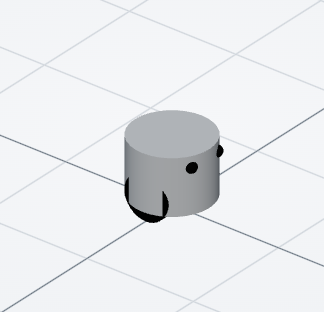
\includegraphics[width=0.8\textwidth, height=0.85\textheight, keepaspectratio]{pictures/robot_perspective.png}
    \caption{Simplified model of an e-Puck 2 as cylinder body with differential wheels. Eyes added purely for aesthetics.} 
    \label{fig:sim:robot}
\end{figure}

The arena (Figure \ref{fig:sim:arena}) for the task consist of two rooms separated by the wall. Each room has different coloured floor so the robot is able to different between them using only its sensors. 
In the separating wall there is a contrasting door. The door swings open on the push of the robot. 
Robot's task originate in orange room, then in second room, the blue one, there is contrasting post, which robot is supposed to reach.

\begin{figure}[htbp]
    \centering
    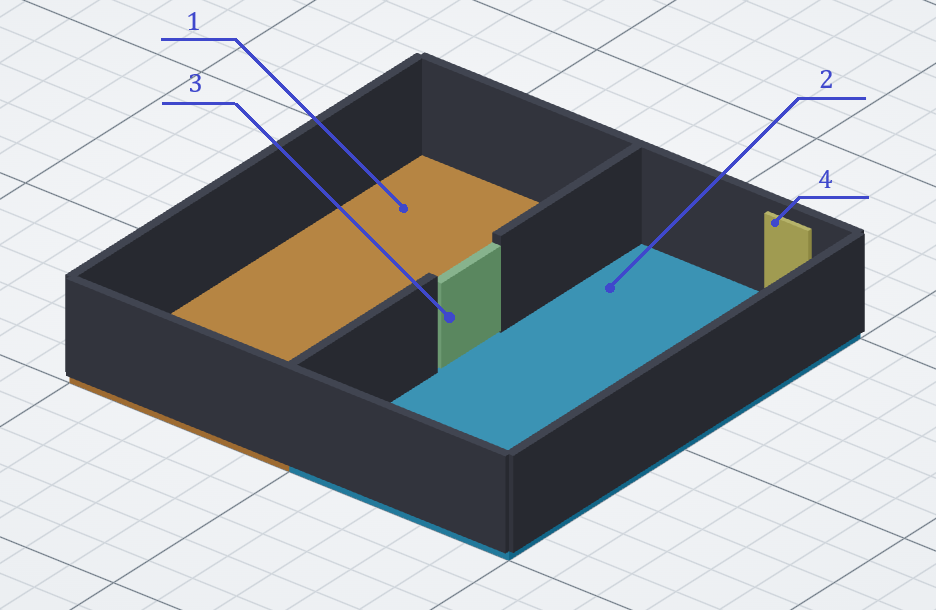
\includegraphics[width=0.8\textwidth, height=0.85\textheight, keepaspectratio]{pictures/arena_perspective.png}
    \caption{Model of an arena used in the simulation. Two rooms separated by a wall with the door.} 
    \label{fig:sim:arena}
\end{figure}

\subsection{Supervisor}
Next module updates the data for all the debugging figures and answers robot's questions through the bus. This is the implementation of supervision within the learning. 
The supervisor has knowledge beyond robot's perception and can modulate both the environment and robot. 
The main task of a supervisor in the learning process is checking if a skill was executed successfully, Each skill has some conditions of success and failure. 
This is similar to what is being learned, but the difference is that those are formulated in terms of the outsider. The outsider can have different sensors or simply different point of reference. 
For example, the supervisor knows in which room the robot is, the robot does not. The skill 'start' can be executed anywhere, has no precondition, but is finished successfully only if the robot is in the orange room.
Supervisor checks this condition and returns to the agent if it succeed.

\subsection{Agent}
This module consist of the main logic loop, the networks for predicates and transitions, and low-level skills. 

\subsubsection*{Predicates} 
Predicates are represented by Supervised Growing Neural Gas. These are implementation of basic GNG \textcite{fritzke1994gng} with added behaviour for negative points. 
The original algorithm was for unsupervised learning, and mapped space from collected points. Since the execution can be successful or not, 
I added a reverse logic for negative points, symmetrical to treating positive ones. If a point considered is positive, the neural gas points are pulled to it. 
If it is negative, they are pushed away. 
\todo{add parameters with explanation for them}

\subsubsection*{Transition graph} 
The transition graph is represented by a standard directed graph. It plays no role in the learning process. This graph is used for generating PDDL files.  
The transitions are collected from the overlapping points of effects and preconditions and generated after each update to either of them.  

\subsubsection*{PDDL files} 
PDDL files are generated by simple, structural code. Each time the predicates are updated, the new problem and domain files are generated. 
The domain file (Listing \ref{lst:pddl:domain}) defines the world for an agent. What can be seen (predicates) and what can be done (actions). In this domain there are as many actions as skills, and for each skill two types of predicates: can-run-skill and executed-skill. This way we cover both starting conditions for a skill and its effect.
The problem file (Listing \ref{lst:pddl:problem}) specify the domain and the predicates that are fulfilled at the beginning and the predicates that need to be fulfilled at the end.
   
\begin{lstlisting}[caption={Problem definition in PDDL}, label={lst:pddl:problem}]
(define (problem plan_problem)
  (:domain robot_domain)
  (:init
    (can_run_Start)
  )
  (:goal
    (executed_Finish)
  )
)
\end{lstlisting}
\begin{lstlisting}[caption={Domain definition in PDDL}, label={lst:pddl:domain}]
(define (domain robot_domain)
  (:requirements :strips)
  (:predicates
    (can_run_Open_the_Door)
    (executed_Open_the_Door)
    (can_run_Start)
    (executed_Start)
    (can_run_Finish)
    (executed_Finish)
    (can_run_Go_to_the_Goal)
    (executed_Go_to_the_Goal)
    (can_run_Go_to_the_Door)
    (executed_Go_to_the_Door)
    (can_run_Find_the_Door)
    (executed_Find_the_Door)
    (can_run_Find_the_Goal)
    (executed_Find_the_Goal)
  )

  (:action Open_the_Door
    :parameters ()
    :precondition (can_run_Open_the_Door)
    :effect (and (executed_Open_the_Door) (can_run_Find_the_Door) (can_run_Find_the_Goal) (not (can_run_Open_the_Door)))
  )

  (:action Start
    :parameters ()
    :precondition (can_run_Start)
    :effect (and (executed_Start) (can_run_Find_the_Door) (not (can_run_Start)))
  )

  (:action Finish
    :parameters ()
    :precondition (can_run_Finish)
    :effect (and (executed_Finish) (not (can_run_Finish)))
  )

  (:action Go_to_the_Goal
    :parameters ()
    :precondition (can_run_Go_to_the_Goal)
    :effect (and (executed_Go_to_the_Goal) (can_run_Finish) (can_run_Find_the_Door) (can_run_Find_the_Goal) (not (can_run_Go_to_the_Goal)))
  )

  (:action Go_to_the_Door
    :parameters ()
    :precondition (can_run_Go_to_the_Door)
    :effect (and (executed_Go_to_the_Door) (can_run_Open_the_Door) (can_run_Find_the_Door) (not (can_run_Go_to_the_Door)))
  )

  (:action Find_the_Door
    :parameters ()
    :precondition (can_run_Find_the_Door)
    :effect (and (executed_Find_the_Door) (can_run_Go_to_the_Door) (not (can_run_Find_the_Door)))
  )

  (:action Find_the_Goal
    :parameters ()
    :precondition (can_run_Find_the_Goal)
    :effect (and (executed_Find_the_Goal) (can_run_Go_to_the_Goal) (not (can_run_Find_the_Goal)))
  )
)
\end{lstlisting}

\subsubsection*{Visual Preprocessing}

\subsubsection*{Low-level Skills}
% Results: some nice graphs and stats
\newpage
\section{Results} \label{chapter:results}

The main goal of the experiments on the described framework is to learn symbols that represent a given environment in terms that are functional for a given robot. Appendix~\ref{app:symbols} holds all learned symbols for a chosen set of hyperparameters.

\subsection{Experiments}

Experiments explored the influence of hyperparameters on learning symbols. They affect the symbols as well as the learning process. Table \ref{tab:experiments} shows the results of varying one parameter while keeping the rest at their defaults. Defaults were chosen arbitrary based on a problem dimentionality, the learning method and a given environment. Their values are shown in table \ref{tab:hyperparam}. 

Each experiment was composed of 10 epochs, 100 runs each. An epoch start in randomly selected place in the room~1 (fig. \ref{fig:sim:arena}, (1)). A run is a full main loop execution (figure \ref{fig:flow_mainloop}), therefore it is an exploration or plan execution, if such is available. Each experiment is concluded with 10 tests. Each test starts in room~1, plans and failing points are collected. 

%TODO: zmienić na tablekę taką jak parametry, żeby się dzieliło na strony
\begin{table}[htbp]
    \centering
    \caption{
        Experiments conducted regarding the influence of Growing Neural Gas (GNG) and symbol abstraction hyperparameters on the resulting symbolic representations and learning process.
        \begin{tabularx}{\textwidth}{@{}l@{\hskip 6pt}X}
            where: & \textbf{parameter} is the parameter and its value that differs from default, \\
                            & \textbf{no. symbols} is the total number of learn symbols, \\
                            & \textbf{run time} is the total time of the experiment, \\
                            & \textbf{success rate} in tests (single run without learning), \\
                            & \textbf{learning drop} how much less the robot learns in next epoch. Since robot collects only unexpected or experimental data, the update frequency should drop with time, 
        \end{tabularx}
    }
    \label{tab:experiments}
  \adjustbox{max width=\textwidth, max totalheight=0.85\textheight, keepaspectratio}
    {
        \begin{tabularx}{\textwidth}{@{} X | X | X | X | X @{}}
            \toprule
            \textbf{parameter} & \textbf{no. symbols} & \textbf{run time} & \textbf{success rate} & \textbf{learning drop} \\
            \hline
            \\
            \bottomrule
        \end{tabularx}
    }
\end{table}



\subsection{Symbols}
\subsubsection*{Perception of the Robot}

\subsubsection*{Symbol Visualisation}
% Discussion: did I succeed? what does it mean?
\newpage
% discussion
\section{Discussion} \label{chapter:discussion}
% skills set is extremely important;
% there is a lot of supervising
% hyperparameters is be or not to be, not just worst/better
% the plan evaluation would be needed: 
% A. if plan did not succeed there is some problem with overlapping method, exp. increase/decrease min_overlap_ratio for this pair; 
% B. connect init and eff nodes; exlude both if next action has a problem ??? but then it should know the correct order a priori
% for this to be more usefull, the sesnsors should be seperated, like distance and colors is two different GNGs -> could be accomplished by analisis of invariants in existing ones?
% symbols accomplished, they look sensible, but its just the translation between supervisor and robot :(
% it get stuck in the conners and has no way to escape.

% Extras: thanks and AI disclosure
\newpage
\textbf{Acknowledgements}\\

\textbf{AI}\\


% --- Apendices ---
\appendix
\newpage
\section{Symbolic representations.} \label{app:symbols}

% --- Helper Functions ---
\newcommand{\skillFigure}[3]{%
  % #1: Human-readable Skill Name (e.g. Finish)
  % #2: File type (e.g. precondition -> init, effect -> eff)
  % #3: symbol type (e.g. precondition, effect)
  \StrSubstitute{#1}{_}{ }[\skillname]
  \begin{figure}[htbp]
    \centering
    \begin{subfigure}[b]{0.9\textwidth}
      \centering
      \includegraphics[width=\linewidth]{pictures/#1_#2_icon.png}
      \caption{Iconic representation}
    \end{subfigure}\hfill
    \begin{subfigure}[b]{0.9\textwidth}
      \centering
      \includegraphics[width=\linewidth]{pictures/#1_#2_invariants.png}
      \caption{Categorical representation}
    \end{subfigure}
    \caption{'\skillname' skill #3 symbolic representation. Two types of visualising obtained symbol: iconic and categorical.}
  \end{figure}
}

\foreach \skill in {Start, Find_the_Door, Go_to_the_Door, Open_the_Door, Find_the_Goal, Go_to_the_Goal, Finish} {
    \skillFigure{\skill}{init}{precondition}
    \skillFigure{\skill}{eff}{effect}
}


\newpage
% Bibliografia
\printbibliography

\end{document}
